\documentclass[oneside,a4paper,titlepage]{scrartcl} % Format fuer Titelseite und Dokument (Koma-Script)
\usepackage[ngerman]{babel}                         % Sprache
\usepackage[utf8]{inputenc}                         % Direkte Angabe von Umlauten Dokument
\usepackage{graphicx}                               % Bilder
\usepackage{listings}                               % Aufzaehlungen
\usepackage{xcolor}                                 % Farbgebung des Sourcodes
\usepackage{lmodern}                                % Formatierung des Sourcecodes
\usepackage{longtable}                              % Fuer mehrseitige Tabellen
\usepackage{booktabs}                               % Fuer mehrseitige Tabellen
\usepackage{colortbl}                               % Fuer farbige Zeilen/Reihen in Tabellen

% Formatierung fuer Sourcecode
\DeclareFontShape{OT1}{cmtt}{bx}{n}{<5><6><7><8><9><10><10.95><12><14.4><17.28><20.74><24.88>cmttb10}{}
\definecolor{eclipse-violet}{rgb}{0.50,0.0,0.46}
\definecolor{eclipse-green}{rgb}{0.25,0.50,0.37}
\definecolor{eclipse-blue}{rgb}{0.17,0.0,1.00}
\lstset{
 language=C++, % Fuer C++ Coding-Style
 showstringspaces=false,
 basicstyle=\ttfamily\small,
 keywordstyle=\bfseries\color{eclipse-violet},
 commentstyle=\color{eclipse-green},
 stringstyle=\color{eclipse-blue}
}

% Beginn des Dokuments
\begin{document}
 
% Titelseite aufbauen
%\titlehead{\flushright
\includegraphics[scale=.3]{img/HAW_logo.png}}
\subject{Software Engineering II\\Wintersemester 2014/2015}
\title{Requirements and Design Documentation}
\subtitle{Praktikums-Gruppe: 2.3}

% Titelseite: Autoren aufbauen
\author{
\begin{small}
 \begin{tabular}{|l|l|c|p{6cm}|}
  \hline
  \textbf{Name} & \textbf{Vorname} & \textbf{Matrikel-Nr.} & \textbf{E-Mail}\\
  \hline
  Kirstein & Katja & 2125137 & katja.kirstein@haw-hamburg.de\\
  \hline
  Kowalka & Anne-Lena & 2081899 & anne-lena.kowalka@haw-hamburg.de\\
  \hline
  Triebe & Marian & 2124897 & marian.triebe@haw-hamburg.de\\
  \hline
  Winter & Eugen & 2081992 & eugen.winter@haw-hamburg.de\\
  \hline
 \end{tabular}
\end{small}
}

% Titelseite: Versionshistorie aufbauen
\publishers{
\begin{small}
 \begin{tabular}{|c|c|c|p{6cm}|}
  \hline
  \textbf{Version} & \textbf{Autor} & \textbf{Datum} & \textbf{Anmerkungen}\\
  \hline
  0.1 & Thomas Lehmann & 17.09.2014 & Überarbeitung des Templates\\
  \hline
  0.2 & Anne-Lena Kowalka & 07.10.2014 & Use Cases samt Diagramm, Require-ments und Arbeitspakete hinzugefügt\\
  \hline
  0.3 & Eugen Winter & 16.10.2014 & Abnahmetests hinzugefügt\\
  \hline
  0.4 & Eugen Winter & 02.11.2014 & RDD als \LaTeX -Dokument erstellt\\
  \hline
  0.5 & Anne-Lena Kowalka & 05.11.2014 & Diverse Updates, Softwarearchitektur konkretisiert (Komponentendiagramm), Testprotokoll hinzugef\"ugt \\
  \hline
 \end{tabular}
\end{small}
}

% Titelseite mit Datum und Version erstellen und Seitenzahl bei 1 beginnen
\date{\today\thanks{Dokument-Version: 0.5}} % ! Hier die Versionsnummer an Versionshistorie anpassen !
\maketitle
\setcounter{page}{1}

% Inhaltsverzeichnis anlegen
\tableofcontents

\newpage

% 1. Motivation
\section{Motivation}
Es gilt, eine Werkstück-SortierAnlage zu programmieren. Die Anlage besteht aus zwei
Förderbändern, die durch eine serielle Schnittstelle miteinander verbunden sind und jeweils durch
einen eigenen GEME-Rechner angesteuert werden.
Es gibt drei Werkstücke unterschiedlicher Art (flach, mit Bohrung und Metall, mit Bohrung ohne
Metall). Am Ende von Band 2 sollen nur normal hohe Werkstücke mit Bohrung nach oben
ankommen, wobei sich Werkstücke mit bzw. ohne Metall abwechseln.

% 2. Teamorganisation
\section{Team-Organisation}

% 2.1 Verantwortlichkeiten
\subsection{Verantwortlichkeiten}
Entscheidungen werden gemeinsam im Team gefällt.\newline
Ansprechpartner gesamtes Team: Eugen Winter\newline
Github-Verwaltung: Marian Triebe\newline
Protokollführerin: Anne-Lena Kowalka\newline
RDD-Führerin: Anne-Lena Kowalka\newline
Implementierung: Katja Kirstein, Anne-Lena Kowalka, Marian Triebe, Eugen Winter\newline
Testen: Katja Kirstein, Anne-Lena Kowalka, Marian Triebe, Eugen Winter\newline

% 2.2 Absprachen
\subsection{Absprachen}
\textbf{Termin für Meetings:} Freitags 14:00 (Stand: 26.9.2014)\newline
\textbf{Weitere Termine:} Nach Absprache

\newpage

% 3. Projektplan
\section{Projektplan}

% 3.1 PSP/Zeitplan/Tracking
\subsection{PSP/Zeitplan/Tracking}
\textbf{Verwendetes Vorgangsmodell:} V-Modell\newline
\newline
\textbf{Festgestellte Arbeitspakete mit ihrer zugehörigen Dauer (Stand: 7.10.2014):}\newline
\newline
 \begin{small}
  \begin{tabular}{|p{8cm}|p{5cm}|}
   \hline
   \rowcolor{gray}\textbf{Arbeitspaket} & \textbf{Dauer}\\
   \hline
   Requirements feststellen & 5h insgesamt\\
   \hline
   Use Cases feststellen & 5h insgesamt\\
   \hline
   RDD bearbeiten & 2h/Woche\\
   \hline
   Git-Repository-Verwaltung & 1h/Woche\\
   \hline
   Codequalität sicherstellen & 1h/Woche\\
   \hline
   Schnittstellenansteuerung/Interface & 3h insgesamt\\
   \hline
   Projektplanung mit GanttProject/MS Project & 3h insgesamt\\
   \hline
   Regressionstests & 8h insgesamt\\
   \hline
   Protokollführung & 1h/Woche\\
   \hline
   Meetings abhalten & 1.5h/Woche\\
   \hline
   Moderation der Meetings/Agenda erstellen & 30 Min/Meeting bzw. Woche\\
   \hline
   UML-Diagramme erstellen & 8h insgesamt\\
   \hline
   HAL bzw. Ports ansteuern (Tasten, Lichter, serielle Schnittstelle, Sensorik) & 20h insgesamt\\
   \hline
   Tests & 16h insgesamt\\
   \hline
   Fehlerbehandlung/-korrektur & 30h insgesamt\\
   \hline
  \end{tabular}
\end{small}

% 3.2 Repository-Konzept
\subsection{Repository-Konzept}
Coding Style: Google C++ Style Guide, konkrete Beschreibung im Anhang\newline
Branching Strategie: Auf dem \emph{master} Branch befindet sich nur der aktuelle Milestone.\newline
Aktuelle Entwicklungen finden auf dem \emph{develop} Branch statt.\newline
Es gibt die Möglichkeit Feature-Branches auf Basis des \emph{develop} Branches zu erstellen.

% 3.3 Qualitätssicherung
\subsection{Qualitätssicherung}
Durch Testen nach jeder Phase, bzw. Unit-Tests, soll die Qualität sichergestellt werden.

\newpage

% 4. Randbedingungen
\section{Randbedingungen}

% 4.1 Entwicklungsumgebung
\subsection{Entwicklungsumgebung}
Momentics IDE für QNX, Doxygen

% 4.2 Werkzeuge
\subsection{Werkzeuge}
\textbf{Betriebssystem:} QNX und QNX-VM mit SEAP Simulation\newline
\textbf{Hardware:} GEME Embedded Controller

% 4.3 Sprachen
\subsection{Programmier-Sprachen}
C++ (nur STL)

% 5. Requirements und Use Cases
\section{Requirements und Use Cases}

% 5.1 Stakeholder
\subsection{Stakeholder}
\begin{itemize}
    \item Entwickler
    \item Tester
    \item Kunde
    \item Betreuer
    \item Personal
\end{itemize}

\newpage

% 5.2 Anforderungen
\subsection{Anforderungen}

% 5.2.1 Funktionale Anforderungen
\subsubsection{Funktionale Anforderungen}
\begin{small}
 \begin{longtable}{|p{2cm}|p{4cm}|p{1.5cm}|p{5.5cm}|}
  \hline
  \textbf{ID} & \textbf{Titel} & \textbf{Bereich} & \textbf{Beschreibung}\\
  \toprule
  \endhead
  \hline
  FR-001 & Typen von Werkstücken & Werkstück & Es gibt 3 Typen von Werkstücken:Zu flach, mit Bohrung, sowie mit und ohne Metalleinsatz.\\
  \hline
  \rowcolor{gray} FR-002 & Anzahl der Sortierbänder & Anlage & Für die Werkstück-Sortieranlage stehen 2 Sortierbänder zur Verfügung.\\
  \hline
  FR-003.1 & Ziel der Werkstück-Sortieranlage & Anlage & Am Ende von Band 2 sollen die Werkstücke im Wechsel mit und ohne Metalleinsatz ankommen.\\
  \hline
  FR-003.2 & Ziel der Werkstück-Sortieranlage & Anlage & Am Ende von Band 2 sollen die einzelnen Werkstücke mit der Bohrung nach oben liegend ankommen.\\
  \hline
  \rowcolor{gray} FR-004 & Zuführung eines Werk-stücks in die Werkstück-Sortieranlage & Anlage & Das Werkstück wird vom Personal an den Anfang von Band 1 in den Bereich der Lichtschranke gelegt.\\
  \hline
  FR-005 & Entnahme eines Werk-stücks aus der Werkstück-Sortieranlage & Anlage & Nach dem erfolgreichen Durchlaufen der Sortieranlage, wird das Werkstück am Ende von Band 2 vom Personal entnommen.\\
  \hline
  \rowcolor{gray} FR-006.1 & Erkennen und Aussortieren von zu flachen Werkstücken & Sensorik & Zu flache Werkstücke werden auf Band 1 mit Hilfe der Höhenmessung erkannt.\\
  \hline
  \rowcolor{gray} FR-006.2 & Erkennen und Aussortieren von zu flachen Werkstücken & Anlage & Nach der Erkennung werden zu flache Werkstücke auf Band 1 mit Hilfe der Weiche aussortiert.\\
  \hline
  FR-007.1 & Erkennen und Ausrichten verkehrt liegender Werkstücke & Sensorik & Mit Hilfe der Höhenmessung erkennt Band 1, ob ein Werkstück mit der Bohrung nach oben oder unten auf das Band gelegt wurde.\\
  \hline    
  FR-007.2 & Erkennen und Ausrichten verkehrt liegender Werkstücke & Anlage & Das verkehrt liegende Werkstück mit der Bohrung nach unten wird an das Ende von Band 1 befördert und die Anlage hält an.\\
  \hline
  FR-007.3 & Erkennen und Ausrichten verkehrt liegender Werkstücke & Anzeige & Die gelbe Signalleuchte der Ampelanlage von Band 1 signalisiert mit einem Blinken dem Personal, dass ein Wenden des Werkstücks notwendig ist.\\
  \hline    
  FR-007.4 & Erkennen und Ausrichten verkehrt liegender Werkstücke & Sensorik & Ein Timer wird beim Eintreten in den wartenden Zustand gestartet und räumt dem Personal zum Wenden des Werkstücks eine vordefinierte Zeitspanne ein.\\
  \hline    
  FR-007.5 & Erkennen und Ausrichten verkehrt liegender Werkstücke & Personal & Das Personal wendet das Werkstück von Hand mit der Bohrung nach oben, quittiert den Hinweis und startet die Anlage wieder.\\
  \hline    
  FR-007.6 & Erkennen und Ausrichten verkehrt liegender Werkstücke & Fehler & Es kommt zu einer Fehlermeldung, wenn das Werkstück nicht innerhalb der vordefinierten Zeitspanne wieder zurück auf das Ende von Band 1 gelegt worden ist.\\
  \hline
  \rowcolor{gray} FR-008.1 & Erkennen und Aussortieren verkehrt liegender Werkstücke & Sensorik & Mit Hilfe der Höhenmessung erkennt Band 2, ob ein Werkstück mit der Bohrung nach unten auf dem Band liegt.\\
  \hline    
  \rowcolor{gray} FR-008.2 & Erkennen und Aussortieren verkehrt liegender Werkstücke & Anlage & Nach Erkennung eines verkehrt liegenden Werkstücks auf Band 2, wird dieses mit Hilfe der Weiche aussortiert.\\
  \hline
  FR-009.1 & Einhalten der korrekten Reihenfolge der Werk-stücke & Sensorik & Mit Hilfe des Metallsensors auf Band 2 wird erkannt, ob hintereinander zwei gleichartige Werkstücke (mit/ohne Metalleinsatz) befördert worden sind.\\
  \hline    
  FR-009.2 & Einhalten der korrekten Reihenfolge der Wer-kstücke & Anlage & Nach Erkennung der falschen Reihenfolge wird das betroffene Werkstück an den Anfang von Band 2 befördert.\\
  \hline
  FR-009.3 & Einhalten der korrekten Reihenfolge der Werk-stücke & Anzeige & Die gelbe Signalleuchte der Ampelanlage von Band 2 signalisiert mit einem Blinken dem Personal, dass ein Entfernen des Werkstücks notwendig ist.\\
  \hline
  FR-009.4 & Einhalten der korrekten Reihenfolge der Werk-stücke & Personal & Das Personal entfernt das betroffene Werkstück von Hand, quittiert den Hinweis und startet die Anlage erneut.\\
  \hline
  \rowcolor{gray} FR-010 & Hinzufügen von Werk-stücken auf Anfang von Band 1 & Anlage & Es dürfen, sobald der Anfang mit der Lichtschranke von Band 1 frei ist, weitere Werkstücke auf den Anfang von Band 1 gelegt werden.\\
  \hline
  FR-011 & Anzahl der Werkstücke auf Band 1 & Anlage & Es dürfen sich mehrere Werkstücke zeitgleich auf Band 1 befinden.\\
  \hline
  \rowcolor{gray} FR-012.1 & Übergabe von Werk-stücken von Band 1 an Band 2 & Anlage & Die Werkstücke von Band 1 werden einzeln an Band 2 übergeben, wenn dieses frei ist.\\
  \hline    
  \rowcolor{gray} FR-012.2 & Übergabe von Werk-stücken von Band 1 an Band 2 & Anlage & Es darf sich nur ein Werkstück zeitgleich auf Band 2 befinden.\\
  \hline
  FR-013 & Identifizieren eines Werk-stücks & Werkstück & Jedes Werkstück bekommt intern nach der Vermessung auf Band 1 eindeutige Werkstück-Eigenschaften zugewiesen.\\
  \hline
  \rowcolor{gray} FR-014 & Zusammensetzung der Werkstück-Eigenschaften & Anlage & Die Werkstück-Eigenschaften beinhalten: ID aus fortlaufender Zahl, Typ des Werkstücks (zu flach, mit Metalleinsatz, ohne Metalleinsatz, Bohrung nach oben, Bohrung nach unten) und den Höhenmesswerten von Band 1 und Band 2.\\
  \hline
  FR-015 & Ausgeben der Werkstück-Eigenschaften & Anlage & Wenn ein Werkstück das Ende von Band 2 erreicht hat, werden die ID, der Typ und die Höhenmesswerte von Band 1 und Band 2 auf der Konsole ausgegeben.\\
  \hline
  \rowcolor{gray} FR-016 & Ampelanlage & Anzeige & Die Werkstück-Sortieranlage besitzt an beiden Bändern jeweils eine Ampelanlage, mit der sich der Betriebszustand des jeweiligen Bandes und der gesamten Anlage abbilden lässt.\\
  \hline
  FR-017 & Grüne Signalleuchte & Anzeige & Die grüne Signalleuchte der jeweiligen Ampelanlage signalisiert den fehlerfreien Betrieb.\\
  \hline
  \rowcolor{gray} FR-018.1 & Gelbe Signalleuchte & Anzeige & Die gelbe Signalleuchte von Band 1 signalisiert einen Hinweis an das Personal das Werkstück von Hand mit der Bohrung nach oben zu drehen.\\
  \hline
  \rowcolor{gray} FR-018.2 & Gelbe Signalleuchte & Anzeige & Die gelbe Signalleuchte von Band 2 signalisiert einen Hinweis an das Personal das Werkstück vom Ende des Bandes zu entfernen.\\
  \hline
  FR-019.1 & Rote Signalleuchte & Anzeige & Die Anlage besitzt eine rote Signalleuchte um zu signalisieren, dass ein Fehler aufgetreten ist: Rutsche voll; zu lange Laufzeit; zu kurze Laufzeit.\\
  \hline
  FR-019.2 & Rote Signalleuchte & Anzeige & Ein nicht quittierter Fehler lässt die rote Signalleuchte schnell blinken (1Hz).\\
  \hline
  FR-019.3 & Rote Signalleuchte & Anzeige & Die Quittierung eines Fehlers ändert das Blinken der roten Signalleuchte in ein Dauerlicht.\\
  \hline
  FR-019.4 & Rote Signalleuchte & Anzeige & Ein Fehler, der verschwunden ist oder sich von selbst gelöst hat, lässt die rote Signalleuchte langsam blinken (0.5Hz).\\
  \hline
  FR-019.5 & Rote Signalleuchte & Anzeige & Solange keine Fehler aufgetreten sind, ist die rote Signalleuchte erloschen.\\
  \hline
  \rowcolor{gray} FR-020 & Ruhezustand & Anlage & Befinden sich keine Werkstücke auf den Bändern, sollen diese angehalten werden.\\
  \hline
  FR-021 & Verschwinden von Werk-stücken & Fehler & Bei zu langen Laufzeiten zwischen den Lichtschranken liegt ein Verschwinden des Werkstücks vor. Es wird eine Fehlermeldung ausgegeben und die Anlage stoppt.\\
  \hline
  \rowcolor{gray} FR-022 & Hinzufügen von Werk-stücken mitten auf dem Band & Fehler & Bei zu kurzen Laufzeiten zwischen den Lichtschranken wurde ein Werkstück mitten auf das Band gelegt. Es wird eine Fehlermeldung ausgegeben und die Anlage stoppt.\\
  \hline
  FR-023 & Rutsche voll & Fehler & Bei zu vielen Werkstücken in der Rutsche für die Aussortierung fehlerhafter Werkstücke wird eine Fehlermeldung ausgegeben und die Anlage gestoppt.\\
  \hline
  \rowcolor{gray} FR-024.1 & Ansteuerung der Weiche & Weiche & Die Weiche ist im geschlossenen Zustand stromlos und führt Strom, wenn sie geöffnet ist.\\
  \hline
  \rowcolor{gray} FR-024.2 & Ansteuerung der Weiche & Gefahr & Eine dauerhaft geöffnete Weiche muss aufgrund von Überhitzung des Motors vermieden werden!\\
  \hline
  FR-025 & Not-Aus der Anlage & Gefahr & Die Anlage darf erst nach einem Reset und einem erneuten Starten durch den Start-Taster wieder in Betrieb gehen und nicht bereits nach der Behebung des Fehlers!\\
  \hline
  \rowcolor{gray} FR-026 & Bandlaufgeschwindigkeit bei Höhenmessung & Sensorik & Bei der Höhenmessung auf Band 1 und Band 2 werden die Werkstücke im langsamen Modus des Bandes befördert.\\
  \hline
  FR-027 & Start-Taster & Taster & Die Anlage besitzt einen Start-Taster samt zugehöriger Leuchte zum Einschalten der Anlage.\\
  \hline
  \rowcolor{gray} FR-028 & Stop-Taster & Taster & Die Anlage besitzt einen Stop-Taster samt zugehöriger Leuchte zum Ausschalten der Anlage.\\
  \hline
  FR-029.1 & Reset-Taster & Taster & Die Anlage besitzt einen Reset-Taster samt zugehöriger Leuchte zur Quittierung von Fehlern im Betrieb der Anlage.\\
  \hline
  FR-029.2 & Reset-Taster & Taster & Jeder Fehler muss zuerst quittiert werden. Erst dann kann der Betrieb durch das Betätigen des Ein-Tasters wieder aufgenommen werden.\\
  \hline
  \rowcolor{gray} FR-030.1 & E-Stopp-Taster & Taster & Die Anlage besitzt einen E-Stopp-Taster samt zugehöriger Leuchte zur Schnellabschaltung und Stilllegung der gesamten Werkstück-Sortieranlage.\\
  \hline
  \rowcolor{gray} FR-030.2 & E-Stopp-Taster & Taster & Der E-Stopp-Taster ist LOW-aktiv.\\
  \hline
 \end{longtable} 
\end{small}

% 5.2.2 Nicht-funktionale Anforderungen
\subsubsection{Nicht-funktionale Anforderungen}
\begin{small}
 \begin{longtable}{|p{2cm}|p{4cm}|p{1.5cm}|p{5.5cm}|}
  \hline
  \textbf{ID} & \textbf{Titel} & \textbf{Bereich} & \textbf{Beschreibung}\\
  \toprule
  \endhead
  \hline
  NFR-001 & Timer für das Wenden eines Werkstücks am Ende von Band 1 & Sensorik & Nachdem erkannt wird, dass ein Werkstück mit der Bohrung nach unten auf Band 1 liegt, wird es in die Lichtschranke am Ende von Band 1 gefahren und es läuft ein Timer für 60 Sekunden. In dieser Zeit muss das Werkstück vom Personal gewendet werden, ansonsten wird eine Fehlermeldung ausgelöst.\\
  \hline
  \rowcolor{gray} NFR-002 & Timer für das Entfernen eines Werkstücks in falscher Reihenfolge am Anfang von Band 2 &  Sensorik & Nachdem das korrekt sortierte Werkstück in falscher Reihenfolge auf Band 2 erkannt wurde, fährt es in die Lichtschranke am Anfang von Band 2 zurück und es läuft ein Timer für 60 Sekunden. In dieser Zeit muss das Werkstück vom Personal entfernt werden, ansonsten wird eine Fehlermeldung ausgelöst.\\
  \hline
  NFR-003 & Timer für das Entfernen eines korrekt sortierten Werkstücks am Ende von Band 2 & Sensorik & Nachdem das korrekt sortierte Werkstück das Ende der Lichtschranke von Band 2 erreicht hat, läuft ein Timer für 60 Sekunden. In dieser Zeit muss das Werkstück vom Personal entfernt werden, ansonsten wird eine Fehlermeldung ausgelöst.\\
  \hline
  \rowcolor{gray} NFR-004.1 & Timer für die Beförderung eines Werkstücks durch die Werkstück-Sortieranlage & Sensorik & Ein korrektes Werkstück durchläuft die einzelnen Bänder der Werkstück-Sortieranlage jeweils innerhalb eines Intervalls von 4-5 Sekunden.\\
  \hline
  \rowcolor{gray} NFR-004.2 & Timer für die Beförderung eines Werkstücks durch die Werkstück-Sortieranlage & Sensorik & Eine Laufzeitmessung durch die Lichtschranken von weniger als 4-5 Sekunden bedeutet, dass ein weiteres Werkstück unter Fremdeinwirkung auf das Band gelegt worden ist. Das Band wird angehalten und es wird eine Fehlermeldung ausgelöst.\\
  \hline
  \rowcolor{gray} NFR-004.3 & Timer für die Beförderung eines Werkstücks durch die Werkstück-Sortieranlage & Sensorik & Eine Laufzeitmessung durch die Lichtschranken von mehr als 4-5 Sekunden bedeutet, dass ein Werkstück unter Fremdeinwirkung vom Band entfernt worden ist. Das Band wird angehalten und es wird eine Fehlermeldung ausgelöst.\\
  \hline
  NFR-005 & Timer für das Hinzufügen neuer Werkstücke auf Band 1 & Sensorik & Nachdem ein Werkstück in die Lichtschranke am Anfang von Band 1 gelegt worden ist und das Band läuft, startet ein Timer für 3 Sekunden. In dieser Zeit darf kein neues Werkstück in die Lichtschranke am Anfang von Band 1 gelegt werden, da sonst ein reibungsloser Betrieb nicht mehr garantiert ist. Ansonsten wird eine Fehlermeldung ausgelöst.\\
  \hline
  \rowcolor{gray} NFR-006.1 & Toleranz für die Höhe eines Werkstücks & Sensorik & Die Toleranz für die Höhe eines zu flachen Werkstücks liegt bei 10-15 Millimetern.\\
  \hline
  \rowcolor{gray} NFR-006.2 & Toleranz für die Höhe eines Werkstücks & Sensorik & Die Toleranz für die Höhe eines Werkstücks mit Bohrung nach oben liegt bei 20-30 Millimetern.\\
  \hline
  \rowcolor{gray} NFR-006.3 & Toleranz für die Höhe eines Werkstücks & Sensorik & Die Toleranz für die Höhe eines Werkstücks mit Bohrung nach unten liegt bei 25-30 Millimetern.\\
  \hline
  NFR-007 & Öffnungsdauer der Weiche & Sensorik & Für das Durchlassen korrekter Werkstücke wird die Weiche für 2 Sekunden lang geöffnet.\\
  \hline
 \end{longtable} 
\end{small}

\newpage

% 5.3 Use Cases
\subsection{Use Cases}

\subsubsection{UC1}
\begin{tabbing}
 Links \= Mitte \= Rechts \kill
 \textbf{Titel:} \> \> Akzeptiertes Werkstück\\
 \textbf{Akteur:} \> \> Personal\\
 \textbf{Ziel:} \> \> Werkstück kommt am Ende von Band 2 an\\
 \textbf{Auslöser:} \> \> Ein Werkstück wird in die Lichtschranke am Anfang von Band 1 gelegt. B[0]=0\\
\end{tabbing}
\textbf{Vorbedingung:}
\begin{enumerate}
 \item Laufband 1 befindet sich im Betriebszustand
 \item Die Lichtschranke am Anfang von Band 1 ist frei. B[0]=1
\end{enumerate}
\textbf{Nachbedingung:}
\begin{itemize}
    \item Keine
\end{itemize}
\textbf{Erfolgsszenario:}
\begin{enumerate}
 \item Dem Werkstück wird eine ID vergeben
 \item Die Höhe des Werkstückes wird durch den Höhenmesser ermittelt. B[1]=0
 \item Die Höhe des Werkstücks ist im Toleranzbereich. B[1]=1
 \item Die Weiche des ersten Bandes wird geöffnet und das Werkstück durchgelassen. B[2]=0 und B[5]=1
 \item Die Weiche wird geschlossen. B[5]=0
 \item Das Werkstück kommt auf Band 2, wenn dieses frei ist
 \item Der Typ des Werkstücks wird festgelegt. Das Werkstück mit Bohrung nach oben und mit Metalleinsatz, bzw. ohne Metalleinsatz wird im Wechsel akzeptiert.\\
       (Metall-Kunststoff oder Kunststoff-Metall)
 \item Die Weiche wird geöffnet und das Werkstück durchgelassen. B[2]=0 und B[5]=1
 \item Die Weiche wird geschlossen. B[5]=0
 \item Das Werkstück erreicht die Lichtschranke am Ende von Band 2. B[7]=0
 \item Laufband 2 bleibt stehen
 \item Das Werkstück wird vom Personal entfernt. B[7]=1
\end{enumerate}
\newpage
\textbf{Fehlerszenario:}
\begin{enumerate}
 \item Das Werkstück liegt nicht im Toleranzbereich der Höhe und wird aussortiert.
 \item Die Kommunikation zwischen beiden Laufbändern funktioniert nicht.
 \item Die Reihenfolge der Werkstücke ist falsch.
 \item Werkstücke werden mitten im Betrieb hinzugefügt oder weggenommen.
\end{enumerate}

\subsubsection{UC2}
\begin{tabbing}
 Links \= Mitte \= Rechts \kill
 \textbf{Titel:} \> \> Nicht akzeptiertes Werkstück (zu flach)\\
 \textbf{Akteur:} \> \> -\\
 \textbf{Ziel:} \> \> Werkstücke die zu flach sind, werden von Band 1 aussortiert\\
 \textbf{Auslöser:} \> \> Höhenmesser ermittelt die Höhe des Werkstücks. B[2]\\
\end{tabbing}
\textbf{Vorbedingung:}
\begin{enumerate}
 \item Laufband 1 befindet sich im Betriebszustand
 \item Eingelegtes Werkstück ist zu flach
\end{enumerate}
\textbf{Nachbedingung:}
\begin{itemize}
 \item Aussortiertes Werkstück liegt in der Rutsche
\end{itemize}
\textbf{Erfolgsszenario:}
\begin{enumerate}
 \item Die Höhe des Werkstückes wird durch den Höhenmesser ermittelt. B[1]=0
 \item Das Werkstück ist zu flach. B[2]=1
 \item Die Weiche bleibt im geschlossenen Zustand. B[5]=0
 \item Das Werkstück wird aussortiert
\end{enumerate}
\textbf{Fehlerszenario:}
\begin{enumerate}
 \item Rutsche ist voll
 \item Werkstück bleibt in der Lichtschranke hängen
\end{enumerate}

\subsubsection{UC3}
\begin{tabbing}
 Links \= Mitte \= Rechts \kill
 \textbf{Titel:} \> \> Nicht akzeptiertes Werkstück auf Band 1 (Bohrung nach unten)\\
 \textbf{Akteur:} \> \> Personal\\
 \textbf{Ziel:} \> \> Werkstück am Ende von Band 1 wird mit der Bohrung nach oben umgedreht\\
 \textbf{Auslöser:} \> \> Höhenmesser ermittelt die Höhe des Werkstücks. B[2]\\
\end{tabbing}
\textbf{Vorbedingung:}
\begin{enumerate}
 \item Laufband 1 befindet sich im Betriebszustand
 \item Es befindet sich ein Werkstück auf Band 1
\end{enumerate}
\textbf{Nachbedingung:}
\begin{itemize}
 \item Ein Werkstück befindet sich am Laufbandende
\end{itemize}
\textbf{Erfolgsszenario:}
\begin{enumerate}
 \item Die Höhe des Werkstückes wird durch den Höhenmesser ermittelt. B[1]=0
 \item Ein Werkstück mit Bohrung nach unten wird erkannt
 \item Die Weiche wird geöffnet und das Werkstück durchgelassen. B[2]=0 und B[5]=1
 \item Das Werkstück wird am Ende von Band 1 von der Lichtschranke registriert
 \item Das Laufband bleibt stehen und die gelbe Signalleuchte blinkt. A[6]=1
 \item Das Personal dreht das Werkstück per Hand mit der Bohrung nach oben um
\end{enumerate}

\newpage

\subsubsection{UC4}
\begin{tabbing}
 Links \= Mitte \= Rechts \kill
 \textbf{Titel:} \> \> Rutsche voll\\
 \textbf{Akteur:} \> \> Personal\\
 \textbf{Ziel:} \> \> Rutsche wieder frei. B[6]=1\\
 \textbf{Auslöser:} \> \> Sensorik erkennt, dass die Rutsche voll ist. B[6]=0\\
\end{tabbing}
\textbf{Vorbedingung:}
\begin{enumerate}
 \item Laufband befindet sich im Betriebszustand
 \item Die Rutsche ist voll
\end{enumerate}
\textbf{Nachbedingung:}
\begin{enumerate}
 \item Die Rutsche ist wieder frei für mindestens ein Werkstück
 \item Das Laufband befindet sich im Betriebszustand. B[6]=1 und A[5]=1
\end{enumerate}
\textbf{Erfolgsszenario:}
\begin{enumerate}
 \item Laufband bleibt stehen. Rote Signalleuchte blinkt schnell (1Hz) $\rightarrow$ anstehend unquittiert. A[7]=1
 \item Das Personal drückt den Reset-Taster $\rightarrow$ LED Resettaste leuchtet nicht mehr. C[1]=0
 \item Rote Signalleuchte leuchtet (Dauerlicht) $\rightarrow$ anstehend quittiert. A[7]=1
 \item Das Personal leert die Rutsche. B[6]=1
 \item Das Personal bestätigt die Leerung der Rutsche durch Drücken des Start-Tasters
 \item Anlage läuft wieder $\rightarrow$ Rote Signalleuchte erlischt, grüne Signalleuchte leuchtet. A[7]=0 und A[5]=1
\end{enumerate}
\textbf{Fehlerszenario:}
\begin{enumerate}
 \item Das Personal leert die Rutsche, aber quittiert den Fehler nicht
 \item Der Start-Taster wird nicht nach Leerung der Rutsche gedrückt
 \item Der Fehler wird quittiert und die Anlage gestartet, ohne dass die Rutsche geleert wurde
\end{enumerate}

\newpage

\subsubsection{UC5}
\begin{tabbing}
 Links \= Mitte \= Rechts \kill
 \textbf{Titel:} \> \> Verschwinden von Werkstücken\\
 \textbf{Akteur:} \> \> Personal\\
 \textbf{Ziel:} \> \> Das Fehlen des erfassten Werkstückes wird durch die Anlage signalisiert\\
 \textbf{Auslöser:} \> \> Das Programm meldet zu lange Laufzeiten zwischen Lichtschranken\\
\end{tabbing}
\textbf{Vorbedingung:}
\begin{enumerate}
 \item Laufband befindet sich im Betriebszustand
 \item Ein Werkstück wird vom Band entfernt
\end{enumerate}
\textbf{Nachbedingung:}
\begin{itemize}
 \item Laufband läuft wieder (nur die grüne Signalleuchte leuchtet). A[5]=1
\end{itemize}
\textbf{Erfolgsszenario:}
\begin{enumerate}
 \item Laufband bleibt stehen. Rote Signalleuchte blinkt schnell (1 Hz) $\rightarrow$ anstehend unquittiert. A[7]=1
 \item Das Personal drückt den Reset-Taster $\rightarrow$ LED Resettaste leuchtet nicht mehr. C[1]=0
 \item Rote Signalleuchte leuchtet nicht mehr.
 \item Das Personal betätigt den Start-Taster.
 \item Anlage läuft wieder $\rightarrow$ Grüne Signalleuchte leuchtet. A[7]=0 und A[5]=1
\end{enumerate}

\subsubsection{UC6}
\begin{tabbing}
 Links \= Mitte \= Rechts \kill
 \textbf{Titel:} \> \> Hinzufügen von Werkstücken mitten auf dem Band\\
 \textbf{Akteur:} \> \> Personal\\
 \textbf{Ziel:} \> \> Das nicht erfasste Werkstück wird entfernt\\
 \textbf{Auslöser:} \> \> Das Programm meldet zu kurze Laufzeiten zwischen Lichtschranken\\
\end{tabbing}
\textbf{Vorbedingung:}
\begin{enumerate}
 \item Laufband befindet sich im Betriebszustand
 \item Ein Werkstück wird mittendrin auf das Band gelegt
\end{enumerate}
\textbf{Nachbedingung:}
\begin{itemize}
 \item Laufband läuft wieder (nur die grüne Signalleuchte leuchtet). A[5]=1
\end{itemize}

\newpage

\textbf{Erfolgsszenario:}
\begin{enumerate}
 \item Laufband bleibt stehen. Rote Lampe blinkt schnell (1 Hz) $\rightarrow$ anstehend unquittiert. A[7]=1
 \item Personal drückt den Reset-Taster $\rightarrow$  LED Resettaste leuchtet nicht mehr. C[1]=0
 \item Rote Lampe leuchtet (Dauerlicht) $\rightarrow$  anstehend quittiert. A[7]=1
 \item Das Personal entfernt das Werkstück
 \item Das Personal bestätigt das Entfernen des Werkstücks durch Drücken des Start-Tasters
 \item Anlage läuft wieder $\rightarrow$  Rote Signalleuchte erlischt, grüne Signalleuchte leuchtet. A[7]=0 und A[5]=1
\end{enumerate}
\textbf{Fehlerszenario:}
\begin{enumerate}
    \item Personal entfernt das Werkstück nicht
    \item Personal entfernt das falsche Werkstück
\end{enumerate}

\subsubsection{UC7}
\begin{tabbing}
 Links \= Mitte \= Rechts \kill
 \textbf{Titel:} \> \> Zurücksetzen des Laufbands\\
 \textbf{Akteur:} \> \> Personal\\
 \textbf{Ziel:} \> \> Laufband in Ursprungszustand versetzen\\
 \textbf{Auslöser:} \> \> Das Personal betätigt den Reset-Taster. C[6]=1\\
\end{tabbing}
\textbf{Vorbedingung:}
\begin{itemize}
 \item Laufband befindet sich im Betriebszustand
\end{itemize}
\textbf{Nachbedingung:}
\begin{itemize}
 \item Auf der Anlage befindet sich kein Werkstück
\end{itemize}
\textbf{Erfolgsszenario:}
\begin{enumerate}
 \item Das Laufband bleibt stehen
 \item Das Personal entnimmt alle Werkstücke von der Anlage
 \item Das Personal betätigt erneut die Reset-Taste. C[6]=0
 \item Laufband ist Betriebsbereit $\rightarrow$ Grüne Signalleuchte leuchtet. A[5]=1
\end{enumerate}

\subsubsection{UC8}
\begin{tabbing}
 Links \= Mitte \= Rechts \kill
 \textbf{Titel:} \> \> Starten der Anlage nach Schnellabschaltung\\
 \textbf{Akteur:} \> \> Personal\\
 \textbf{Ziel:} \> \> Die gesamte Anlage ist wieder Betriebsbereit\\
 \textbf{Auslöser:} \> \> E-Stopp-Taster wird gedrückt. C[7]=0\\
\end{tabbing}
\textbf{Vorbedingung:}
\begin{itemize}
 \item Anlage ist angeschaltet
\end{itemize}
\textbf{Nachbedingung:}
\begin{itemize}
 \item Laufband ist Betriebsbereit. A[5]=1
\end{itemize}
\textbf{Erfolgsszenario:}
\begin{enumerate}
 \item Die ganze Anlage (Band 1 und Band 2) steht still
 \item Alle Ampeln sind aus
 \item Alle Weichen sind geschlossen
 \item Das Personal drückt den Start-Taster
 \item Die Anlage läuft wieder
\end{enumerate}

% 5.4 Use-Case-Diagramm
\begin{figure}
 \subsection{Use-Case-Diagramm}
 \centering\vfill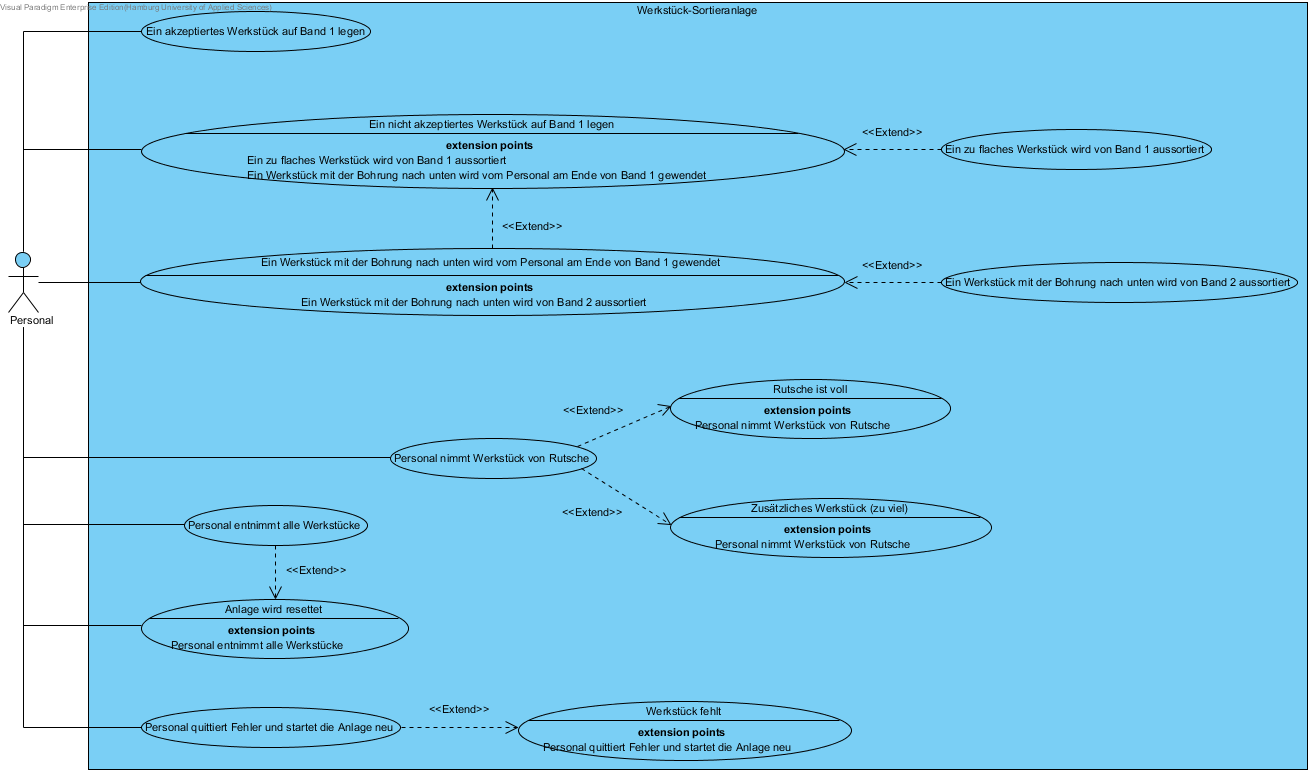
\includegraphics[angle=90,scale=0.7]{uml_imgs/UseCases.png}
\end{figure}

\newpage

% 5.5 Systemanalyse
\subsection{Systemanalyse}
Das System wird \"uber ein C++-Programm gesteuert, welches auf einem (bzw. zwei bei zwei F\"orderb\"andern) Geme-Rechnern l\"auft. Die Aktorik und Sensorik werden \"uber 3 Ports angesteuert, wobei die Sensoren die Werte mittels Interrupts dem System mitteilen.\newline
Die Kommunikation der beiden F\"orderb\"ander l\"auft \"uber eine serielle Schnittstelle. Es werden hier z.B. die Messergebnisse von Band 1 an Band 2 \"ubergeben, damit, wenn ein Puk das Ende von Band 2 erreicht, seine zuge\"origen Daten ausgegeben werden k\"onnen. \newline
\newline
\textcolor{red}{\textbf{Was muss man über das technische System (aus Sicht der zu entwickelnden Software) wissen?
Wie sieht die Struktur aus? Wie der Systemkontext? Welche Schnittstellen betrachten Sie?}}

\newpage

% 6. Design
\section{Design}
\textcolor{red}{\textbf{Anmerkung: Die Implementierung MUSS mit Ihrem Design-Modell korrespondieren.
Daher ist ein wohlüberlegtes Design wichtig.}}

% 6.1 System-Architektur
\subsection{System-Architektur}
Das System verf\"uegt \"ueber folgende Module: HAL zum Ansteuern/Auslesen der Aktorik und Sensorik, Serial Bus zur Ansteuerung der seriellen Schnittstelle, FSM zur Anlagensteuerung und util f\"ur die Thread-Sicherheit(mutex, condvar und lockquard) bzw. f\"ur das Logging. Desweiteren gibt es zugeh\"orige Unit-Tests. \newline
siehe Komponentendiagramm \newline
\textcolor{red}{\textbf{Erstellung der System-Architektur. Geben Sie eine kurze Beschreibung Ihrer
Architektur mit den dazugehörenden Komponenten und Schnittstellen.
Spezifikation der Architektur und Definition der System-Schnittstellen in einem UML Komponentendiagramm.}}

% 6.2 Datenmodell
\subsection{Datenmodell}
siehe Klassendiagramm \newline
\textcolor{red}{\textbf{Bestimmung des Datenmodells mit Hilfe von UML Klassendiagrammen
unter Beachtung der Designprinzipien. Kurze textuelle Beschreibung des Datenmodells und
deren wichtigsten Klassen und Methoden.}}

% 6.3 Verhaltensmodell
\subsection{Verhaltensmodell}
siehe Automatendiagramm \newline
\textcolor{red}{\textbf{Spezifikation der wichtigsten System-Szenarien anhand von Verhaltensdiagrammen.
Sie können für die Spezifikation der Prozess-Lenkung entweder Petri-Netze oder hierarchische Automaten nehmen.}}

\newpage

% 7. Implementierung
\section{Implementierung}
\textcolor{red}{\textbf{Anmerkung: Wichtige Implementierungsdetails sollen hier erklärt werden.
Code-Beispiele (snippets) können hier aufgelistet werden, um der Erklärung zu dienen.
Anmerkung: Bitte KEINE ganze Programme hierhin kopieren!}}

% 7.1 Algorithmen
\subsection{Algorithmen}
\textcolor{red}{\textbf{Wichtige Algorithmen, die Sie hier benutzt haben.}}

% 7.2 Patterns
\subsection{Patterns}
Scope Logging, DCLP, Singelton, Delegator \newline
\textcolor{red}{\textbf{Wichtige Patterns, die Sie implementiert haben.}}

% 7.3 Mapping Rules
\subsection{Mapping Rules}
\textcolor{red}{\textbf{Wichtige Mapping Rules, die Sie benutzt haben, z.B.
um aus Ihrem Design entsprechenden Code zu erstellen.}}

\newpage

% 8. Testen
\section{Testen}
\textcolor{red}{\textbf{Machen Sie sich Gedanken über Unit-Test, Komponententest,
Integrationtest, Systemtest, Regressionstest und Abnahmetest.}}

% 8.1 Unit-Test/Komponenten-Test
\subsection{Unit-Test/Komponenten-Test}
\textcolor{red}{\textbf{Test Szenario eines Laufbands.}}

% 8.2 Integrations-Test/System-Test
\subsection{Integrations-Test/System-Test}
\textcolor{red}{\textbf{Test Szenarien mit beiden Laufbändern.}}

% 8.3 Regressions-Test
\subsection{Regressions-Test}
\textcolor{red}{\textbf{Welche Szenarien müssen immer wieder abgetestet werden? Automatisieren Sie Ihre Tests nach
Möglichkeit}}\\
\newline
\textbf{Mögliche Regressionstests für serielle Schnittstelle:}\\
\begin{enumerate}
 \item Korrektes Telegramm wird übertragen (Länge, Korrektheit)
 \item Fehlerhaftes Telegramm wird übertragen:
 \begin{enumerate}
  \item Ungültige Header-ID
  \item Ungültige Länge (EOF kommt zu früh oder zu spät)
  \item Fehlerhafter Header
  \item Fehlerhafter Inhalt
 \end{enumerate}
 \item Synchronisierung
 \item Höhensensor emulieren
 \item Metallsensor emulieren
\end{enumerate}

% 8.4 Abnahme-Test
\subsection{Abnahme-Test}
Zum Abnahmetest werden alle Requirements und Use Cases durchgegangen. Anschließend werden
die Regressionstests und der Normalbetrieb der Anlage vorgeführt.

% 8.5 Testplan
\subsection{Testplan}
\textcolor{red}{\textbf{Zeitpunkte für die jeweiligen Teststufen in Ihrer Projektplanung setzen.
Dazu können Sie die Meilensteine zu Hilfe nehmen.}}

% 8.6 Testprotokolle und Auswertungen
\subsection{Testprotokolle und Auswertungen}
4.11.2014: Testen der HAL, insbesondere der Sensorik \newline
Nachdem die korrekte Ansteuerung der Aktorik und die serielle Schnittstelle mit dem zweiten Milestone abgenommen wurde, wurde die Sensorik getestet. Es wurde beobachtet, dass der H\"ohensensor (korrekte) Messwerte liefert. Weiterhin wurde beobachtet, dass das Programm sich aufh\"angt, sobald ein Messwert geliefert bzw. ein Interrupt von der Sensorik ausgel\"ost wurde. Dies ben\"otigt weitere Bearbeitung.\newline

\textcolor{red}{\textbf{Hier fügen Sie die Test Protokolle bei, auch wenn Fehler bereits beseitigt
worden sind, ist es schön zu wissen, welche Fehler einst aufgetaucht sind.
Eventuelle Anmerkung zur Fehlerbehandlung kann für weitere Entwicklungen hilfreich sein.\\
Das letzte Testprotokoll ist das Abnahmeprotokoll, das bei der abschließenden Vorführung erstellt
wird. Es enthält eine Auflistung der erfolgreich vorgeführten Funktionen des Systems sowie eine
Mängelliste mit Erklärungen der Ursachen der Fehlfunktionen und Vorschlägen zur Abhilfe}}

% 9. Lessons Learned
\section{Lessons Learned}
\textcolor{red}{\textbf{Was lief gut, was lief schlecht in diesem Projekt (technisch und organisatorisch)?\\
Was haben Sie gelernt?\\
Weitere Anregungen und Erkenntnisse durch das Projekt.}}

\newpage

% 10. Glossar
\section{Glossar}
\textcolor{red}{\textbf{Eindeutige Begriffserklärungen.}}

% 11. Abkürzungen
\section{Abkürzungen}
WS = Werkstück\\
\textcolor{red}{\textbf{Listen Sie alle Abkürzungen auf, die Sie in diesem Dokument benutzt haben.}}

% 12. Anhänge
\section{Anhänge}
\begin{enumerate}
 \item Alle Modell-Dateien (VisualParadigm, Petri-Netze, etc.)
 \item Sourcecode und Code-Dokumentationen (z.B. Doxygen)
 \item Test-Protokolle
 \item Meeting-Protokolle
 \item Projektstruktur
 \item etc.
\end{enumerate}
\textcolor{red}{\textbf{Auflistung aller Artefakten dieses Projekts.}}

\newpage

% 12.1 Coding Style: Google C++
\subsection{Coding Style: Google C++}

% 12.1.1 General Rules
\subsubsection{General Rules}
\begin{itemize}
 \item Use 2 spaces per indentation level.
 \item The maximum number of characters per line is 80.
 \item Never use tabs.
 \item Vertical whitespaces separate functions and are not used inside functions: use comments to document logical blocks.
 \item Header filenames end in \emph{.hpp}, implementation files end in \emph{cpp}.
 \item Never declare more than one variable per line.
 \item Ampersand {\&} binds to the \emph{type}, e.g., \emph{const std::string}\& \emph{arg}.
 \item Namespaces do not increase the indentation level.
 \item Access modifiers, e.g. \emph{public}, are indented one space.
 \item Use the order \emph{public}, \emph{protected}, and then \emph{private}.
 \item Use \emph{typename} only when referring to dependent names.
 \item Keywords are always followed by a whitespace: \emph{if (...), template \textless...\textgreater, while (...)}, etc.
 \item Always use \emph{\{\}} for bodies of control structures such as \emph{if} or \emph{while}, even for bodies consiting only of a single statement.
 \item Opening braces belong to the same line:
 \begin{lstlisting}
if (my_condition) {
  my_fun();
} else {
  my_other_fun();
}
 \end{lstlisting}
 \item Use standard order for readability: C standard libraries, C++ standard libraries, other libraries, your headers:
 \begin{lstlisting}
#include <sys/types.h>
#include <vector>
#include "some/other/library.hpp"
#include "myclass.hpp"
 \end{lstlisting}
 \item When declaring a function, the order of parameters is: outputs, then inputs. This follows the parameter order from the STL.
 \item Never use C-style casts.
\end{itemize}

% 12.1.2 Naming
\subsubsection{Naming}
\begin{itemize}
 \item Class names, constants, and function names are all-lowercase with underscores.
 \item Types and variables should be nouns, while functions performing an action should be "{}command"{} verbs.
       Classes used to implement metaprogramming functions also should use verbs, e.g., \emph{remove\_const}.
 \item Member variables use the prefix \emph{m\_}.
 \item Thread-local variables use the prefix \emph{t\_}.
 \item Static, non-const variables are declared in the anonymous namespace and use the prefix \emph{s\_}.
 \item Template parameter names use CamelCase.
 \item Getter and setter use the name of the member without the \emph{m\_} prefix:
 \begin{lstlisting}
class some_fun {
 public:
  // ...
  int value() const {
    return m_value;
  }
  void value(int new_value) {
    m_value = new_value;
  }
 private:
  int m_value;
};
 \end{lstlisting}
\end{itemize}

% 12.1.3 Headers
\subsubsection{Headers}
\begin{itemize}
 \item Each \emph{.cpp} file has an associated \emph{.hpp} file. Exceptions to this rule are unit tests and \emph{main.cpp} files.
 \item All header files should use \emph{\#define} guards to prevent multiple inclusion.
 \item Do not \emph{\#include} when a forward declaration suffices.
 \item Use \emph{inline} for small functions (rule of thumb: 10 lines or less).
\end{itemize}

\newpage

% 12.1.4 Breaking statements
\subsubsection{Breaking Statements}
\begin{itemize}
 \item Break constructor initializers after the comma, use four spaces for indentation, and place each
 initializer on its own line (unless you don't need to break at all):
 \begin{lstlisting}
my_class::my_class()
    : my_base_class(some_function()),
      m_greeting("Hello there! This is my_class!" ),
      m_some_bool_flag(false) {
  // ok
 }
other_class::other_class() : m_name("tommy"), m_buddy("michael") {
  // ok
 }
 \end{lstlisting}
 \item Break function arguments after the comma for both declaration and invocation:
 \begin{lstlisting}
intptr_t channel::compare(const abstract_channel* lhs,
                          const abstract_channel* rhs) {
  // ...
}
 \end{lstlisting}
 \item Break before tenary operators and before binary operators:
 \begin{lstlisting}
if (today_is_a_sunny_day()
    && it_is_not_too_hot_to_go_swimming()) {
  // ...
}
 \end{lstlisting}
\end{itemize}

\end{document}
}